\chapter{Capacità predittive del modello e applicabilità clinica}\label{ch:predizione}
In questo capitolo sono descritte le capacità \textit{predittive} del modello, ovvero sono quantificati gli errori di simulazione che si commettono quando i parametri del modello utilizzati per simulare una particolare seduta sono ricavati dall'ottimizzazione sulle sedute precedenti dello stesso paziente. Si confronteranno gli errori di descrizione, ricavati nel capitolo precedente (\textit{gold standard}), con quelli di predizione.

\section{Parametri ottimizzati sulla prima seduta}\label{sec:ott1sed}
La \tablename~\ref{tab:pred1} mostra gli errori assoluti $|e_i|$ che si commettono sulla simulazione delle concentrazioni plasmatiche, calcolati in due casi:
\begin{enumerate}
	\item quando le sedute 2, 3 e 4 sono simulate dopo aver ottimizzato i parametri sulle stesse sedute;
	\item quando le sedute del punto precedente sono simulate identificando i parametri sulla seduta 1.
\end{enumerate}
Lo scopo di questo confronto è quello di valutare la possibilità di utilizzare il modello per predire l'andamento di sedute successive alla prima, dopo aver identificato i parametri su un set di dati provenienti dalle sedute precedenti.
Gli errori di predizione sono sempre mediamente più alti rispetto al gold standard, ad eccezione delle proteine e del magnesio in cui questi errori si mantengono sullo stesso livello. Sul caso delle proteine c'è da aggiungere che le ipotesi di simulazione che le riguardano dovranno essere comunque parzialmente riviste.

\begin{table}[htb]
	\centering
	\caption{Errori $|e_i|$ descrittivi a confronto con quelli predittivi sulle sedute 2, 3 e 4. $N_{sample}=65$. I parametri per la predizione sono identificati sui dati della seduta 1.}\label{tab:pred1}
	\begin{tabular}{lrrrrrrrr}
	\toprule 
		\textbf{Soluto}   &    \multicolumn{6}{c}{Errori di simulazione $|e_i|$ ($\%$)}    \\
				              &        \multicolumn{3}{c}{\textbf{descrittivi}}             &       \multicolumn{3}{c}{\textbf{predittivi}}             \\
		                  & \multicolumn{1}{c}{$\mu$}      & \multicolumn{1}{c}{$\sigma$}     & $max$   & \multicolumn{1}{c}{$\mu$}     & \multicolumn{1}{c}{$\sigma$}    & $max$  \\
    \cmidrule(lr){2-4}\cmidrule(lr){5-7}
    %                    media    dev.std.     max     media ass   dev.st.       min       max
  	Sodio             & $0,78$   & $0,48$   & $ 2,12$  & $5,05$   & $3,61$    & $12,93$  \\ 
  	Potassio          & $3,31$   & $3,05$   & $11,86$  & $6,97$   & $4,85$    & $21,73$  \\
  	Cloro             & $0,46$   & $0,38$   & $ 1,82$  & $3,74$   & $2,27$    & $ 8,45$  \\
  	Calcio            & $1,48$   & $1,57$   & $10,62$  & $14,25$  & $10,31$   & $35,38$  \\
  	Fosfato           & $6,69$   & $6,32$   & $32,98$  & $12,41$  & $11,14$   & $37,27$  \\ 
  	Magnesio          & $5,28$   & $4,16$   & $18,23$  & $6,44$   & $3,96$    & $14,90$  \\
  	Urea              & $9,13$   & $6,74$   & $23,34$  & $14,41$  & $9,18$    & $34,92$  \\
  	Creatinina        & $9,21$   & $6,27$   & $26,67$  & $13,01$  & $8,37$    & $35,08$  \\
  	Proteine          & $7,51$   & $4,66$   & $18,55$  & $7,96$   & $4,51$    & $18,48$  \\ 
   	\bottomrule
\end{tabular}
\end{table}	

\begin{figure}[!h]
\centering
		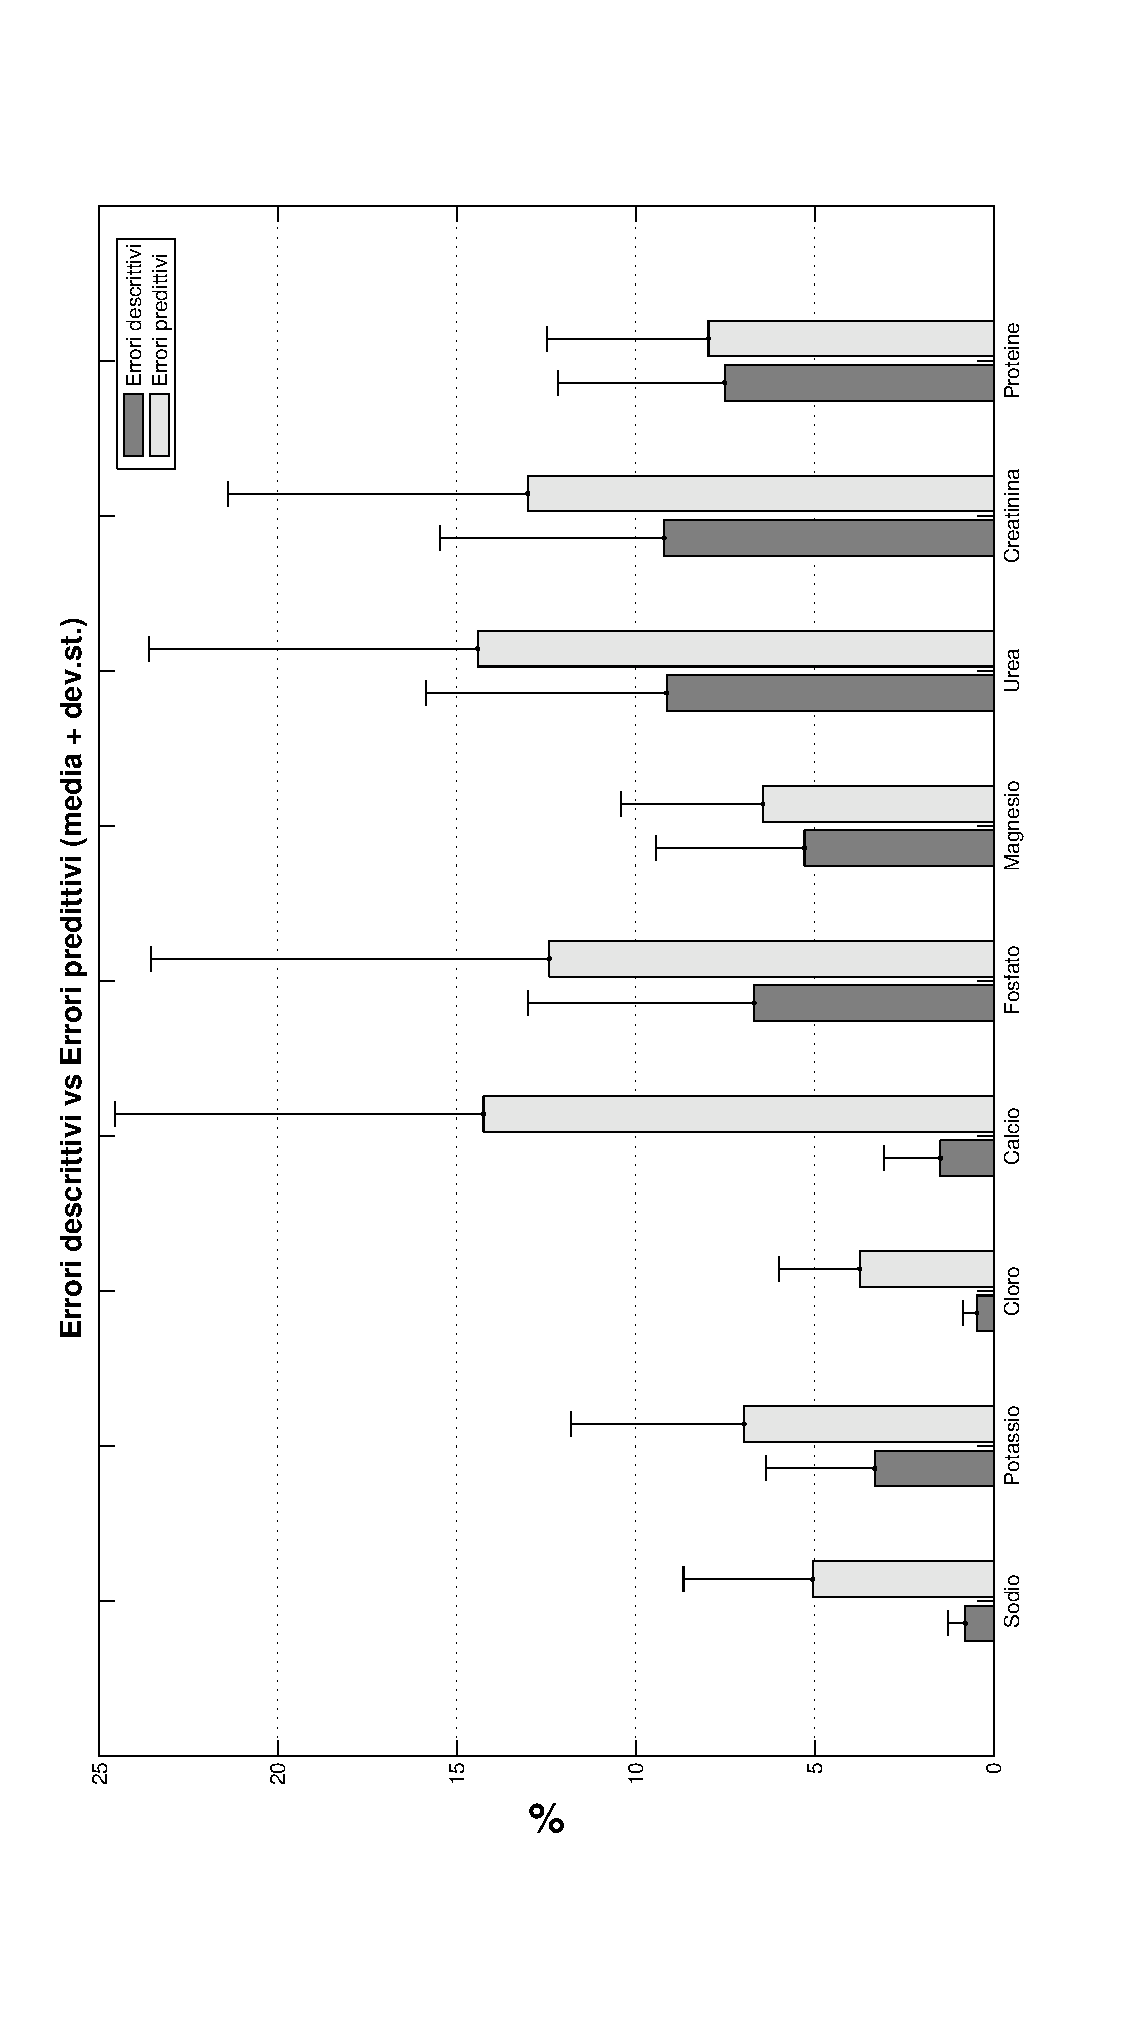
\includegraphics[angle=-90, width=\textwidth]{immagini/desVSpred.eps}
				\caption{Media + deviazione standard degli errori descrittivi confrontati con quelli predittivi (sedute 2, 3 e 4, $N_{sample}=65$). I parametri per la predizione sono stati identificati sulla seduta 1.}\label{fig:desVSpred}
\end{figure}

\begin{description}
	\item[Sodio:] in fase di previsione gli errori di simulazione raggiungono un valore massimo del $21,73\%$, che corrisponde a circa $31$ $mmol/L$ (valore di riferimento $142$ $mmol/L$). Poiché il sodio è il soluto che influisce maggiormente sull'osmolarità plasmatica, gli errori di predizione sul sodio (non tascurabili) potrebbero influenzare la simulazione della dinamica degli altri soluti.
	\item[Potassio:] gli errori di predizione raggiungono un valore massimo del $12,93\%$, che corrisponde a circa $0,5$ $mmol/L$ (rif. $4,2$ $mmol/L$). Se per una valutazione di lungo termine consideriamo i valori medi, allora l'errore di predizione è inferiore alle $0,3$ $mmol/L$.
	\item[Cloro:] in fase di previsione gli errori di simulazione presentano una media del $3,74\%$, che corrisponde a circa $4$ $mmol/L$ (rif. $108$ $mmol/L$). Come per il sodio, anche il cloro ha un effetto importante sull'osmolarità plasmatica, e un errore di simulazione sul cloro potrebbe quindi avere effetti anche sulla simulazione degli altri soluti.
	\item[Calcio:] in questo caso gli scostamenti fra gold standard e predizione sono evidenti. Gli errori medi, infatti, passano da $1,48\%$ al $14,25\%$. Prima di utilizzare il modello sviluppato a scopi predittivi sarebbe opportuno rivedere la modellizzazione del soluto aggiungendo un terzo compartimento. È plausibile pensare ad un buffer identificato dal periostio, lo strato che riveste le ossa, dal quale e verso il quale il calcio può essere velocemente mobilizzato \cite{merulla}.
	\item[Fosfato:] in fase di previsione gli errori di simulazione raggiungono un valore massimo del $37,27\%$, che corrisponde a circa $0,75$ $mmol/L$ (rif. $2$ $mmol/L$). Ricordiamo che il modello per questo soluto dovrebbe essere aggiornato con l'aggiunta di uno o due compartimenti interagenti con quello plasmatico.
	\item[Magnesio:] per questo elettrolita non si notano differenze significative con quanto descritto nel capitolo precedente.
	\item[Urea:] in fase di previsione gli errori di simulazione raggiungono un valore massimo del $34,92\%$, che corrisponde a circa $1,4$ $mmol/L$ (rif. $4$ $mmol/L$). Ipotizzando nel peggiore dei casi che questo sia un errore di sottostima a fine dialisi, e cioé che, basandosi sulla previsione del modello si rischia di mandare a casa il paziente con più urea del previsto, si potrebbe compensare l'incertezza prolungando il tempo di dialisi.
	\item[Creatinina:] in fase di previsione gli errori di simulazione raggiungono un valore massimo del $35,08\%$, che corrisponde a circa $0,07$ $mmol/L$ (rif. $0,2$ $mmol/L$). Anche in questo caso, come per l'urea, si potrebbe pensare, a scopi cautelativi, di prolungare il tempo di dialisi.
\end{description}

\section{Parametri ottimizzati sulle prime due sedute}
La \tablename~\ref{tab:pred2} mostra gli errori assoluti $|e_i|$ che si commettono sulla simulazione delle concentrazioni plasmatiche, calcolati in due casi:
\begin{enumerate}
	\item quando le sedute 3 e 4 sono simulate dopo aver ottimizzato i parametri sulle stesse sedute;
	\item quando le sedute 3 e 4 sono simulate coi parametri identificati e mediati sulle due sedute precedenti.
\end{enumerate}
Lo scopo di questo confronto è quello di valutare la possibilità di utilizzare il modello per poter fare previsioni sulle sedute future, dopo aver identificato i parametri su un set di dati provenienti da due sedute. Come nel caso della predizione basata su un'unico processo identificativo (\textsection~\ref{sec:ott1sed}), gli errori di predizione sono sempre mediamente più alti rispetto al gold standard.

In \figurename~\ref{fig:pred_1vs2} sono messi a confronto gli errori di predizione, commessi dopo l'identificazione dei parametri su una seduta con quelli commessi dopo l'identificazione su due sedute. Si tratta del confronto diretto fra gli errori predittivi di \tablename~\ref{tab:pred1} con quelli di \tablename~\ref{tab:pred2}. Non si notano differenze sostanziali fra gli istogrammi, e sembra quindi che l'identificare i parametri su più di una seduta non comporti miglioramenti sulla predizione delle sedute successive.

\begin{table}[!h]
	\centering
	\caption{Errori $|e_i|$ descrittivi a confronto con quelli predittivi sulle sedute 3 e 4. $N_{sample}=43$. I parametri per la predizione sono identificati sui dati delle seduta 1 e 2 e mediati fra loro.}\label{tab:pred2}
	\begin{tabular}{lrrrrrrrr}
	\toprule 
		\textbf{Soluto}   &    \multicolumn{6}{c}{Errori di simulazione $|e_i|$ ($\%$)}    \\
				              &        \multicolumn{3}{c}{\textbf{descrittivi}}             &       \multicolumn{3}{c}{\textbf{predittivi}}             \\
		                  & \multicolumn{1}{c}{$\mu$}      & \multicolumn{1}{c}{$\sigma$}   & $max$   & \multicolumn{1}{c}{$\mu$}     & \multicolumn{1}{c}{$\sigma$}   & $max$  \\
    \cmidrule(lr){2-4}\cmidrule(lr){5-7}
    
	Sodio      & $0,78$ & $0,52$ & $2,12$  & $4,60$  & $3,55$  & $11,40$ \\ 
	Potassio   & $3,17$ & $2,98$ & $11,86$ & $7,63$  & $7,74$  & $31,82$ \\
	Cloro      & $0,39$ & $0,33$ & $1,62$  & $3,03$  & $2,79$  & $9,55$  \\
	Calcio     & $1,70$ & $1,85$ & $10,62$ & $14,39$ & $14,23$ & $51,90$ \\
	Fosfato    & $6,25$ & $6,73$ & $32,98$ & $16,17$ & $13,12$ & $42,88$ \\
	Magnesio   & $5,33$ & $4,69$ & $18,23$ & $7,24$  & $4,17$  & $14,77$ \\
	Urea       & $8,78$ & $6,60$ & $23,34$ & $13,81$ & $7,83$  & $34,61$ \\
	Creatinina & $8,88$ & $6,00$ & $21,80$ & $12,12$ & $6,49$  & $26,20$ \\
	Proteine   & $8,24$ & $4,56$ & $18,55$ & $8,75$  & $4,15$  & $18,71$ \\
\bottomrule
\end{tabular}
\end{table}
\begin{figure}[!htb]
\centering
		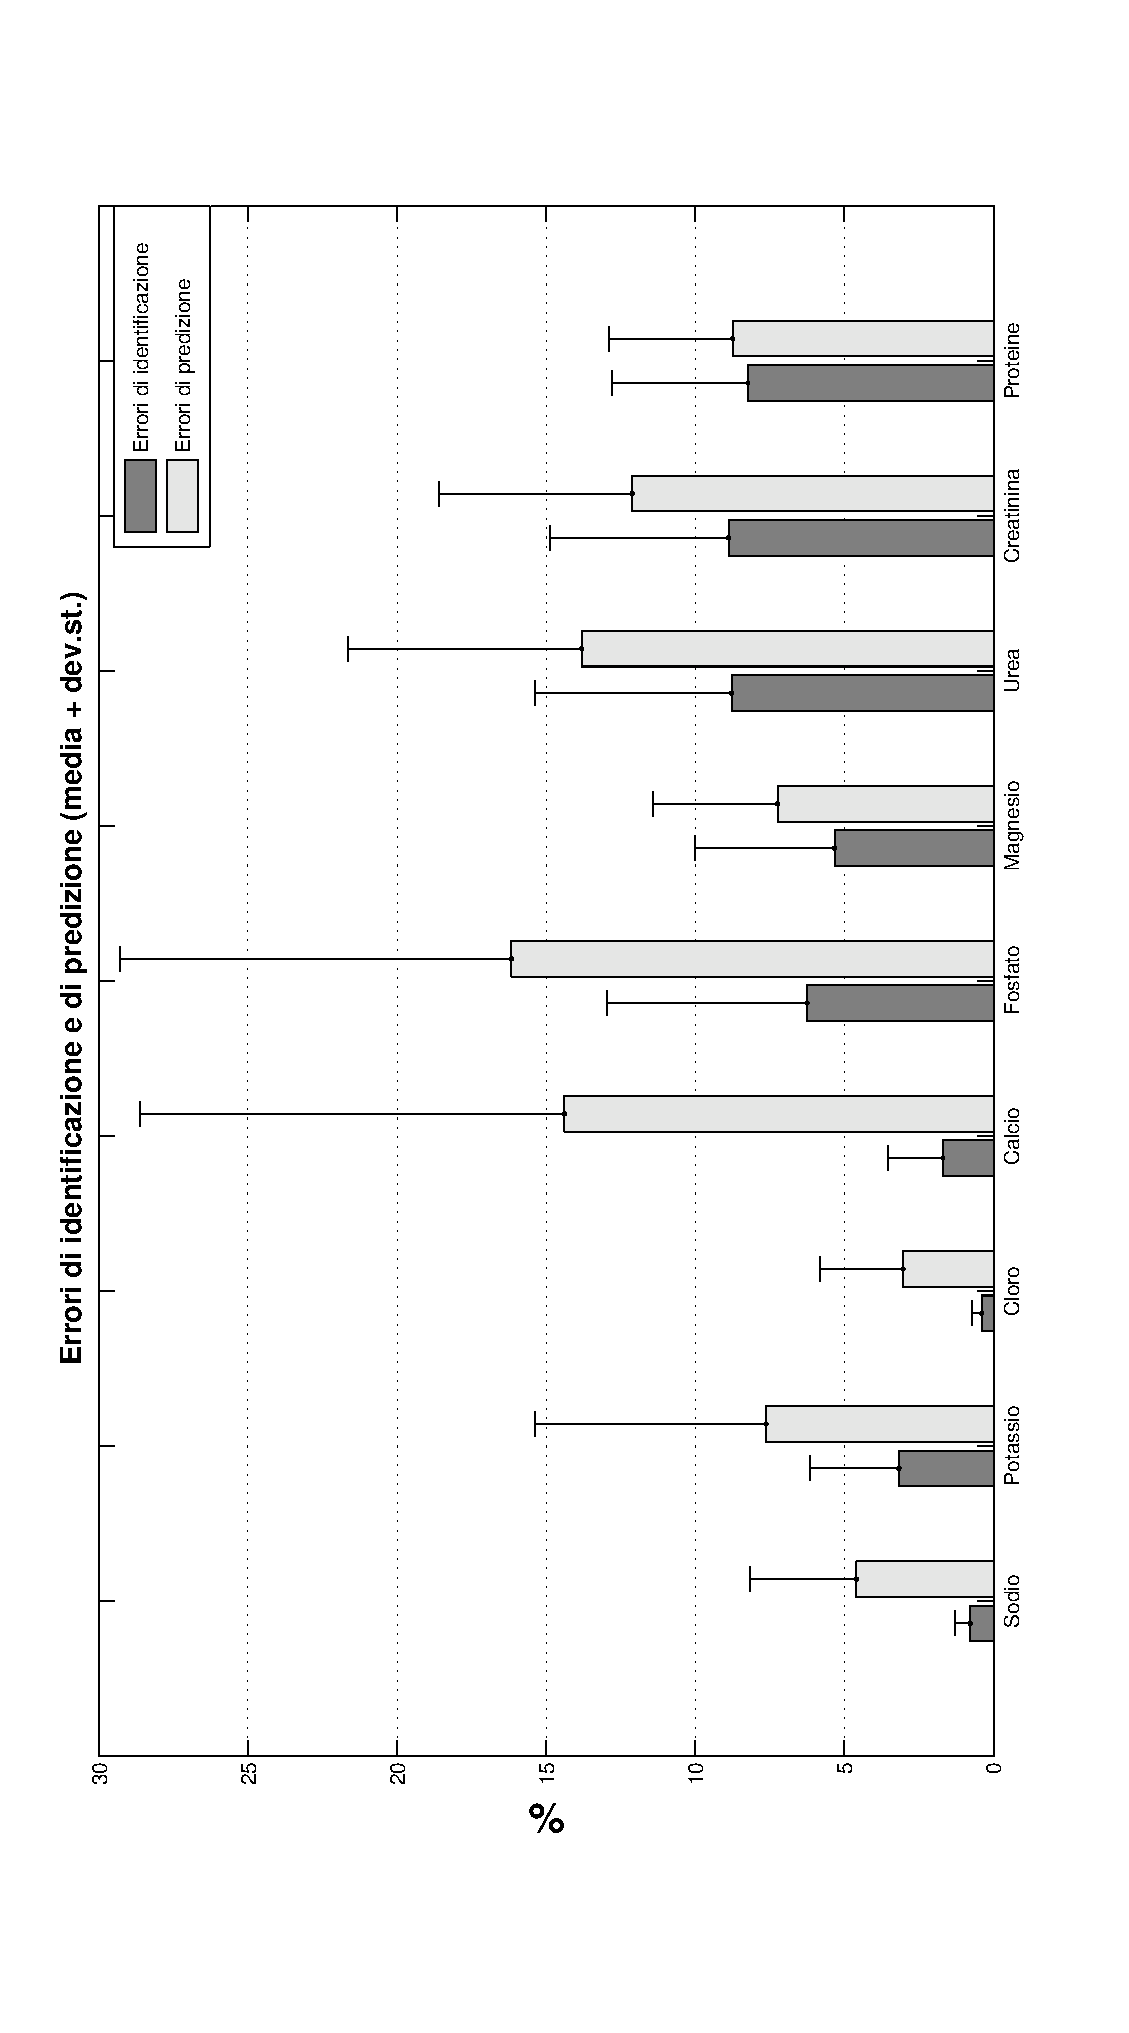
\includegraphics[angle=-90, width=\textwidth]{immagini/desVSpred2.eps}
				\caption{Media + deviazione standard degli errori descrittivi confrontati con quelli predittivi (sedute 3 e 4, $N_{sample}=43$). I parametri per la predizione sono stati identificati e mediati sulle sedute 1 e 2.}\label{fig:desVSpred2}
\end{figure}

\begin{figure}[!htb]
\centering
		\includegraphics[angle=-90, width=\textwidth]{immagini/pred_1vs2.eps}
				\caption{Media + deviazione standard degli errori di predizione. Confronto fra gli errori commessi dopo l'identificazione dei parametri su una seduta e quelli commessi dopo l'identificazione su due sedute. Non si notano differenze sostanziali.}\label{fig:pred_1vs2}
\end{figure}

\section{Applicabilità clinica: pre- \textit{vs} post-diluizione}
Uno degli aspetti più controversi dell'emodiafiltrazione riguarda la modalità di diluizione da utilizzare: pre- o post-diluizione. Entrambe le metodiche possiedeno sia vantaggi che svantaggi (Capitolo~\ref{ch:prepost}), ed è quindi auspicabile capire quale sia quella più adatta a scopi clinici. In post-diluizione è maggiore la clearance delle molecole a basso peso molecolare, ma è anche maggiore il rischio di perdite di albumina a causa delle elevate pressioni di transmembrana. Dall'altra parte, con la pre-diluizione queste perdite di albumina sono scongiurate, ma la clearance dei soluti a basso peso molecolare è ridotta a causa della diluizione a monte del dializzatore (riduzione del gradiente di concentrazione) \cite{masakane, colussi}.

Le sedute simulate in questa tesi sono state effettuate tutte in post-diluizione. Tuttavia nel modello proposto è possibile simulare ambedue le modalità di diluizione, specificandola nei dati in ingresso attraverso una stringa (\verb|type_hdf='pre '| oppure \verb|type_hdf='post'|). In \figurename~\ref{fig:prevspost} è stata simulata la stessa seduta sia in pre- che in post-diluizione. Precisamente la post-diluizione è stata simulata utilizzando come dati in ingresso la media dei dati in ingresso delle $24$ sedute dialitiche seguite nel periodo di studio. Per la simulazione della prediluizione si sono utilizzati gli stessi dati di ingresso, modificando opportunamente la portata di diluizione $Q_s$ in modo da mantenere, in ambedue le simulazioni, la stessa frazione di filtrazione $FF$.
\begin{figure}[tbh]
	\centering
	\advance\leftskip-.2\textwidth
		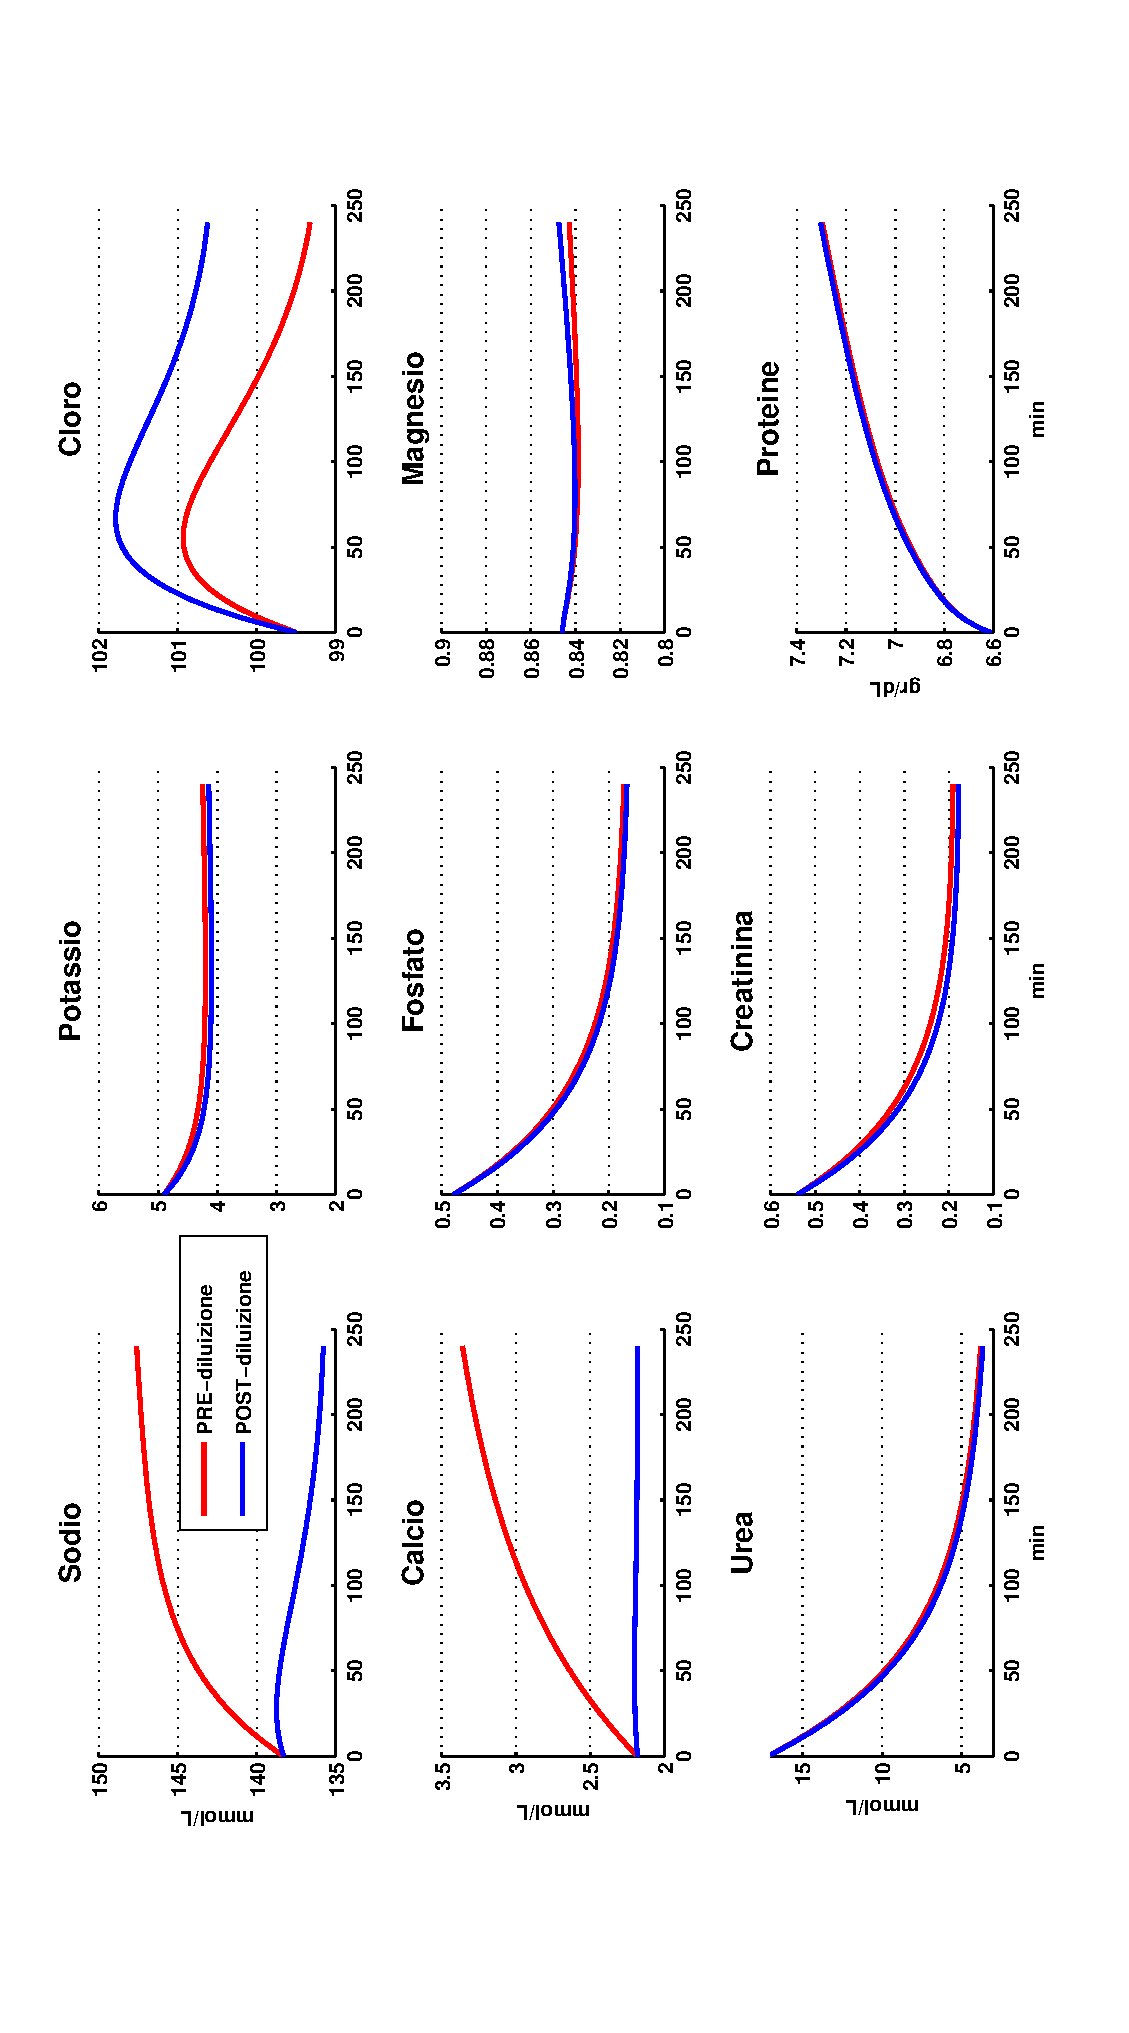
\includegraphics[angle=-90, width=1.4\textwidth]{immagini/prevspost.eps}
		\caption{Confronto fra pre-diluizione (linea rossa) e post-diluizione (linea blu). La seduta dialitica originale è quella in post-diluizione. Per la pre-diluizione sono stati utilizzati gli stessi parametri e le stesse condizioni iniziali della post-diluizione, ad eccezione della portata di infusione $Q_s$ che è stata modificata per ottenere la stessa frazione di filtrazione ($FF$) pari a $0,51$.}\label{fig:prevspost}
\end{figure}
Rispetto a fosfato, magnesio, urea e creatinina (escludendo dall'analisi le proteine per le quali si è ipotizzato che non interagiscono col dializzatore) non si notano differenze significative fra le due modalità. Fra gli elettroliti, il sodio, il cloro e il calcio mostrano una clearance maggiore in post-diluizione, il che è confermato dalla letteratura quando si afferma che i soluti a basso peso molecolare sono meglio rimossi in post-diluizione \cite{masakane}. Il cloro, pur essendo un soluto a basso peso molecolare, mostra però un comportamento opposto agli altri elettroliti. Essendo l'unico elettrolita con carica negativa a mostrare una marcata differenza, si potrebbe pensare di attribuire questa differenza alla carica, ma allora non si spiegherebbe perché il fosfato con tre cariche negative non mostri un simile andamento. Nel caso del fosfato tuttavia le differenze non sono molto marcate, e ciò può essere dovuto alla sua compartimentazione prettamente intracellulare (coeff. $\beta$>1). Dopo queste considerazioni possiamo individuare una teoria che spieghi le differenze fra pre e post-diluizione basata sulla compartimentazione e sulla carica elettrica dei soluti. Le differenze fra pre e post-diluizione possono essere dovute in primo luogo alla compartimentazione, e quindi al coefficiente $\beta$ (Appendice~\ref{sec:beta}). Ad un coefficiente $\beta>1$ corrisponde una compartimentazione prettamente intracellulare e quindi la pre- o la post-diluizione hanno uno scarso effetto nel diluire la concentrazione plasmatica già bassa. Questo è il caso di potassio, fosfato e magnesio. Viceversa, per i soluti con coefficiente $\beta<1$ corrisponde una compartimentazione prettamente extracellulare e pertanto la pre-diluizione ha un effetto maggiore nel diluirne la concentrazione plasmatica. Questo è il caso di sodio, cloro e calcio, che infatti mostrano una differenza marcata fra pre- e post-diluizione.
Fra i soluti con $\beta<1$, la carica elettrica potrebbe determinare quale delle due modalità di diluizione sarà la più efficace nella rimozione del soluto: se positiva (sodio, calcio) la post-diluizione comporta una capacità di estrazione maggiore; viceversa se negativa (cloro) sarà con la pre-diluizione che si avrà una clearance maggiore.

